\textbf{Do heads succeed together?} On 13,602 training and validation states, the marginal product predicted a 14.30\% hit rate for the path taking the top rank in heads one and two. The observed rate was 19.66\% (2,674 hits), or 1.37 times the product estimate. The second head's marginal top-rank accuracy was 28.39\%. Conditional on a first-head top-rank hit, it reached 39.03\% across 6,852 surviving prefixes. The analogous third-head rates were 17.96\% and 37.55\%. The fifth head reached 47.41\% conditional accuracy, but only 424 prefixes survived to that comparison. The dependence is strongest on some paths and leaves fewer examples for estimating deeper factors.


\subsection{Matched-budget replay on MT-Bench}
Each column below gives mean accepted tokens per complete-horizon state at the indicated number of draft nodes. The two calibration measures use one common path pool across budgets. All 80 evaluation questions contributed, with a median of 59 complete states per question and a range of 1 to 59.
\begin{center}
\begin{tabular}{lrrrrrrr}
\toprule
Policy & 8 & 16 & 32 & 63 & 96 & Brier & ECE\\
\midrule
Fixed marginal & 2.106 & 2.314 & 2.486 & 2.634 & 2.704 & 0.02126 & 0.00643\\
Fixed conditional & 2.150 & 2.342 & 2.516 & 2.653 & 2.725 & 0.02112 & 0.00441\\
MEDUSA+ & 2.268 & 2.452 & 2.604 & 2.726 & 2.792 & 0.01839 & 0.00135\\
Direct classifier & 2.269 & 2.455 & 2.605 & 2.730 & 2.791 & 0.01842 & 0.00172\\
Dynamic conditional & 2.268 & 2.451 & 2.607 & 2.731 & 2.794 & 0.01845 & 0.00125\\
\bottomrule
\end{tabular}
\end{center}


The conditional count table beat the marginal fixed tree at all five budgets. Its largest absolute gain occurred at $B=8$, where acceptance rose from 2.106 to 2.150 tokens per state (a 2.10\% relative gain). At the native-sized budget of 63, the fixed gain was $+0.0192$ (95\% paired interval $[0.0063,0.0341]$). MEDUSA+ still had higher acceptance than either fixed tree at every budget. At $B=63$, conditioning the dynamic logistic model changed acceptance from 2.7264 to 2.7306 ($+0.0042$, interval $[-0.0009,0.0090]$). The direct classifier reached 2.7299. These small differences leave the ordering of the dynamic methods uncertain.

\begin{figure}[htbp]
\centering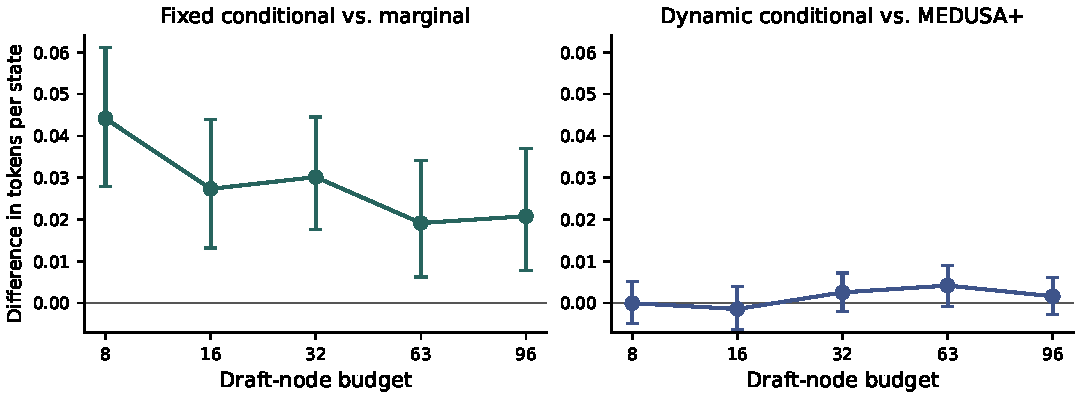
\includegraphics[width=.94\linewidth]{tables/paired_acceptance.pdf}
\caption{Change in accepted tokens per reference state at equal draft budgets. Bars show per-budget 95\% paired prompt-bootstrap intervals. Both panels use the same vertical scale.}
\end{figure}

\textbf{Validation and feature ablation.} Validation selected count smoothing $\alpha=3$, logistic inverse regularization $C=0.1$ and rank cap 4. Enlarging the direct classifier's training pool and adding its own selected nodes did not displace the original 64-node MEDUSA+ pool under the validation selection rule. The conditional logistic model's validation edge Brier score was 0.04566. Removing its confidence features raised the score to 0.04795, the largest change among the seven single-group ablations. Removing the uncertainty features raised it to 0.04597. These are conditional edge scores among accepted parents. The path scores in the main comparison apply to whole prefixes.

\textbf{Path calibration.} On 256,000 evaluation candidate nodes, 2.71\% matched the reference continuation. MEDUSA+ had the lowest Brier score (0.01839). Dynamic conditional regression had the lowest binned ECE (0.00125). Conditional counting improved on the fixed marginal model in both Brier and ECE. Small differences in average probability error need not alter which nodes enter the tree.


\subsection{Live verification and throughput}
\textbf{Reproducing historical precision failures.} The archived Colab run passed its strict check on 15 of 20 pilot prompts and 6 of 7 known cases. The two original detailed JSON reports were unavailable. On the laptop, all seven known cases passed, covering 855 observed rounds of static Medusa and dynamic MEDUSA+ across five budgets. We also reran the five historical pilot failures. Four passed. One of 818 observed rounds across those five prompts failed full-rank equality. At generation offset 19 under $B=32$, the tenth-ranked token of head five changed from ID 310 to 2821. That rank was unused by the selected tree. The largest absolute probability difference across ranked slots in that round was $1.61\times10^{-6}$. Cached and uncached greedy outputs, policy outputs, shared prefixes and selected-node labels all agreed on this subset. The trained head checksum matched the Colab archive. The GPU runtime differed. These observations locate the laptop disagreement. They cannot retrospectively assign a cause to the earlier failures.


On the trained-policy panel, all 80 policy--budget--prompt runs emitted the same token sequence as cached greedy, and every independently rerun greedy sequence matched its saved reference. Across 1,858 complete-horizon live rounds, 182 had at least one candidate-rank difference. Of 332 changed head/rank slots, 104 occurred at ranks used by the tree. Eight of 71,276 selected-node labels disagreed (0.011\%). All eight came from question 141 at generation offset 46 under $B=16$. The first head's sixth- and seventh-ranked tokens traded places for four policies. Each swap reversed one positive and one negative label, so the total number of matching selected nodes agreed in every observed round. These eight errors represent repeated observations of one state. Exact output agreement and agreement in accepted counts can coexist with errors in individual rank-path labels.


\textbf{Measured decoding speed.} The table gives generated tokens per second, throughput divided by cached greedy in the same budget run, and exact output matches out of eight measured questions. Higher throughput is better.
\begin{center}
\begin{tabular}{lrrrrrr}
\toprule
Policy & tok/s$_{16}$ & ratio$_{16}$ & exact & tok/s$_{63}$ & ratio$_{63}$ & exact\\
\midrule
Cached greedy & 9.92 & 1.000 & 8/8 & 10.64 & 1.000 & 8/8\\
Fixed marginal & 9.43 & 0.951 & 8/8 & 8.98 & 0.844 & 8/8\\
Fixed conditional & 9.31 & 0.939 & 8/8 & 8.64 & 0.812 & 8/8\\
MEDUSA+ & 9.60 & 0.968 & 8/8 & 8.85 & 0.832 & 8/8\\
Direct classifier & 9.52 & 0.959 & 8/8 & 8.33 & 0.783 & 8/8\\
Dynamic conditional & 9.40 & 0.947 & 8/8 & 8.26 & 0.776 & 8/8\\
\bottomrule
\end{tabular}
\end{center}


At $B=16$, MEDUSA+ was the fastest speculative policy at 9.60 tokens/s, versus 9.92 for greedy. At $B=63$, the fixed marginal tree led the speculative policies at 8.98 tokens/s, versus 10.64 for greedy. The gain in the fixed conditional tree's offline acceptance did not translate into higher throughput at either budget. On the timed $B=63$ panel, fixed marginal and fixed conditional committed 2.469 and 2.444 tokens per live round, respectively. Both the states visited and the set of prompts differ from full replay.

The separate profile of the first measured prompt at $B=63$ recorded 0.10 ms per round for the fixed conditional tree, 8.06 ms for MEDUSA+ and 20.42 ms for dynamic conditional scoring and buffer handling. At $B=16$ the corresponding values were 0.08, 2.57 and 6.90 ms. This overhead helps explain why the learned dynamic policy can be slower at similar acceptance. The two greedy baselines also differed, which is why each throughput ratio uses the baseline measured within its own budget run.

